% Fig. 3.23 -- the two shapes the event U = X_1 + X_2 <= u takes on the unit
% square, one for each of the two stretches of u.
% Source: mathstatch3.tex lines 5013-5045 (left panel) and 5049-5080 (right
% panel), two tikzpictures set side by side in minipages of .45 and .40 of
% the text width.
%
% Both manuscript panels are kept whole: the outlined unit square, the line
% u = x_1 + x_2 drawn over -1/6 <= x_1 <= 5/6 in the first panel and over
% 1/6 <= x_1 <= 7/6 in the second, the shaded region below that line, the
% marks 0, 1, 1, x_1 and x_2, the label u = x_1 + x_2 on the line and the
% range of u under each panel.  The manuscript's u is 2/3 in the first panel
% and 4/3 in the second; those two values are kept, so the lines cut the
% square exactly where the manuscript has them.  Colours follow
% CH3_FIGURE_SPECS.md section 1.
%
% Three departures from the manuscript:
%
% 1. The panels are stacked rather than set side by side.  This figure sits
%    inside an Example box, whose figure column is 309px on a 390px phone;
%    side by side each panel would get about 150px, and the label
%    u = x_1 + x_2 alone is a quarter of that.  Stacking follows
%    convexity-tangent-lines.tex and jensen-inequality.tex.  Both panels are
%    drawn on one common unit length and one common window, so the two
%    shaded shapes are directly comparable.
%
% 2. The manuscript's \fill in each panel walks out along the plot path and
%    doubles back -- in the first panel out to (0,2) and in the second out to
%    (0,4) in its own units -- which leaves a sliver outside the square.
%    That is an artefact of writing the path through the plot command, not
%    a shape the figure is about, so each region is filled here by its own
%    corners: the triangle (0,0), (0,u), (u,0) in the first panel and the
%    pentagon (0,0), (0,1), (u-1,1), (1,u-1), (1,0) in the second.
%
% 3. The manuscript sets a Chinese 與 between the two minipages to read them
%    as a pair.  Stacked panels do not need it and CH2_FIGURE_SPECS.md 1.4
%    bars Chinese from inside the picture, so it is gone; the caption carries
%    the pairing instead.  The axis names x_1 and x_2 also move against their
%    arrow heads, per CH2_FIGURE_SPECS.md 1.3.
%
% \DeclareMathSizes{12}{12}{10}{9} lifts the math script size from the 8.5pt
% default: the subscripts of x_1 and x_2 are the smallest marks in the
% picture and would otherwise fall under the floor.
%
% Native size 245.662 x 305.042 pt.  A mark of S pt shows at
% S x 0.99626 x <display width> / 245.662 px, so at the 309px phone column
% and the 602px desktop column of a topic-figure--wide inside an Example box:
%     10pt scripts  12.53px (phone)   24.43px (desktop)
%     12pt text     15.04px (phone)   29.31px (desktop)
% At the nominal 350px of the ledger convention the scripts stand at 14.19px.
\documentclass[tikz,border=2pt]{standalone}
\usepackage{amsmath}
\usepackage{amssymb}
\usepackage{xcolor}

\definecolor{journalink}{HTML}{1F1C18}
\definecolor{journalmuted}{HTML}{8A7F72}
\definecolor{journalaccent}{HTML}{9C2D2D}

\DeclareMathSizes{12}{12}{10}{9}

\begin{document}
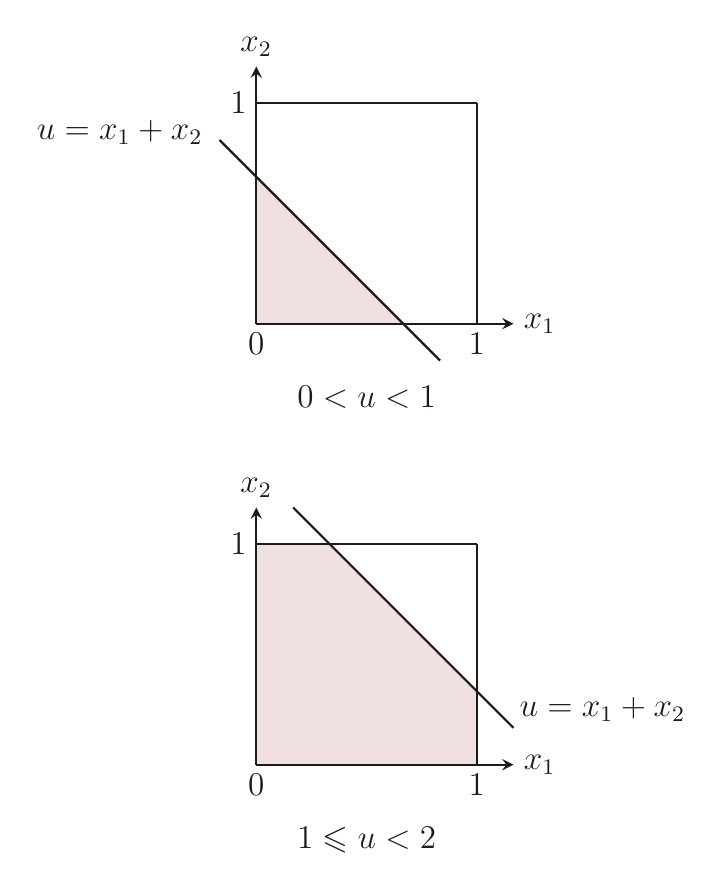
\begin{tikzpicture}[x=2.8cm, y=2.8cm, >=stealth,
                    every node/.style={journalink, font=\large}]

%% ==== 上面板: 0<u<1, 此處書稿取 u = 2/3 =============================
\begin{scope}

  %% U <= u 所對應的三角形
  \fill[journalaccent, fill opacity=0.15] (0,0) -- (0,0.66667) -- (0.66667,0) -- cycle;

  %% 單位正方形的上邊與右邊
  \draw[journalink, line width=0.8pt] (0,1) -- (1,1);
  \draw[journalink, line width=0.8pt] (1,0) -- (1,1);

  %% 界線 u = x_1+x_2
  \draw[journalink, line width=0.8pt] (-0.16667,0.83333) -- (0.83333,-0.16667);

  %% 座標軸
  \draw[journalink, line width=0.8pt, ->] (0,0) -- (1.16667,0) node[right] {$x_1$};
  \draw[journalink, line width=0.8pt, ->] (0,0) -- (0,1.16667) node[above] {$x_2$};

  %% 刻度標示
  \node[below] at (1,0) {$1$};
  \node[below] at (0,0) {$0$};
  \node[left]  at (0,1) {$1$};

  %% 界線的方程式與本面板所處理的 u 範圍
  \node[left]  at (-0.2,0.86667) {$u=x_1+x_2$};
  \node[below] at (0.5,-0.24) {$0<u<1$};

\end{scope}

%% ==== 下面板: 1<=u<2, 此處書稿取 u = 4/3 ============================
\begin{scope}[yshift=-5.6cm]

  %% U <= u 所對應的五邊形, 即單位正方形扣掉右上角的三角形
  \fill[journalaccent, fill opacity=0.15]
    (0,0) -- (0,1) -- (0.33333,1) -- (1,0.33333) -- (1,0) -- cycle;

  %% 單位正方形的上邊與右邊
  \draw[journalink, line width=0.8pt] (0,1) -- (1,1);
  \draw[journalink, line width=0.8pt] (1,0) -- (1,1);

  %% 界線 u = x_1+x_2
  \draw[journalink, line width=0.8pt] (0.16667,1.16667) -- (1.16667,0.16667);

  %% 座標軸
  \draw[journalink, line width=0.8pt, ->] (0,0) -- (1.16667,0) node[right] {$x_1$};
  \draw[journalink, line width=0.8pt, ->] (0,0) -- (0,1.16667) node[above] {$x_2$};

  %% 刻度標示
  \node[below] at (1,0) {$1$};
  \node[below] at (0,0) {$0$};
  \node[left]  at (0,1) {$1$};

  %% 界線的方程式與本面板所處理的 u 範圍。書稿把方程式擺在界線右下端的右方
  %% (3.6, 0.4)，該處與橫軸名稱 $x_1$ 只差 0.4 個單位；本圖的 $x_1$ 貼在箭頭
  %% 上而非書稿的軸線下方，兩者因此只剩 0.05cm，故改標在界線端點的右上方。
  \node[above right, inner sep=2pt] at (1.16667,0.16667) {$u=x_1+x_2$};
  \node[below] at (0.5,-0.24) {$1\leqslant u<2$};

\end{scope}

\end{tikzpicture}
\end{document}
